\task{Фигуры в шахматах}
\begin{itemize}
\itA Какое минимальное количество клеток нужно пройти ферзю из точки $(a,b)$ в точку $(c,d)$ на шахматном поле?

\itB Фигура Корблюд умеет делать из данной клетки на шахматном поле четыре хода так, как показано на рисунке 3. Доказать, что корблюд может прийти из любой клетки бесконечного шахматного поля в любую другую. А верно ли такое утверждение для Корблюда Диагонального, делающего ходы как на рисунке 4?

\itC Будем рассматривать фигуры, которые из данной клетки умеют делать четыре хода: вперёд-налево, вперёд-направо, назад-налево, назад-направо. При этом направо / налево фигура смещается лишь на одну клетку, а вперёд / назад каждый ход — либо на две, либо на три клетки. Сколько фигур, с точностью до симметрий, удовлетворяют этим свойствам, и какие из них могут из любой клетки бесконечного шахматного поля дойти до любой другой?
\end{itemize}

\begin{center}
  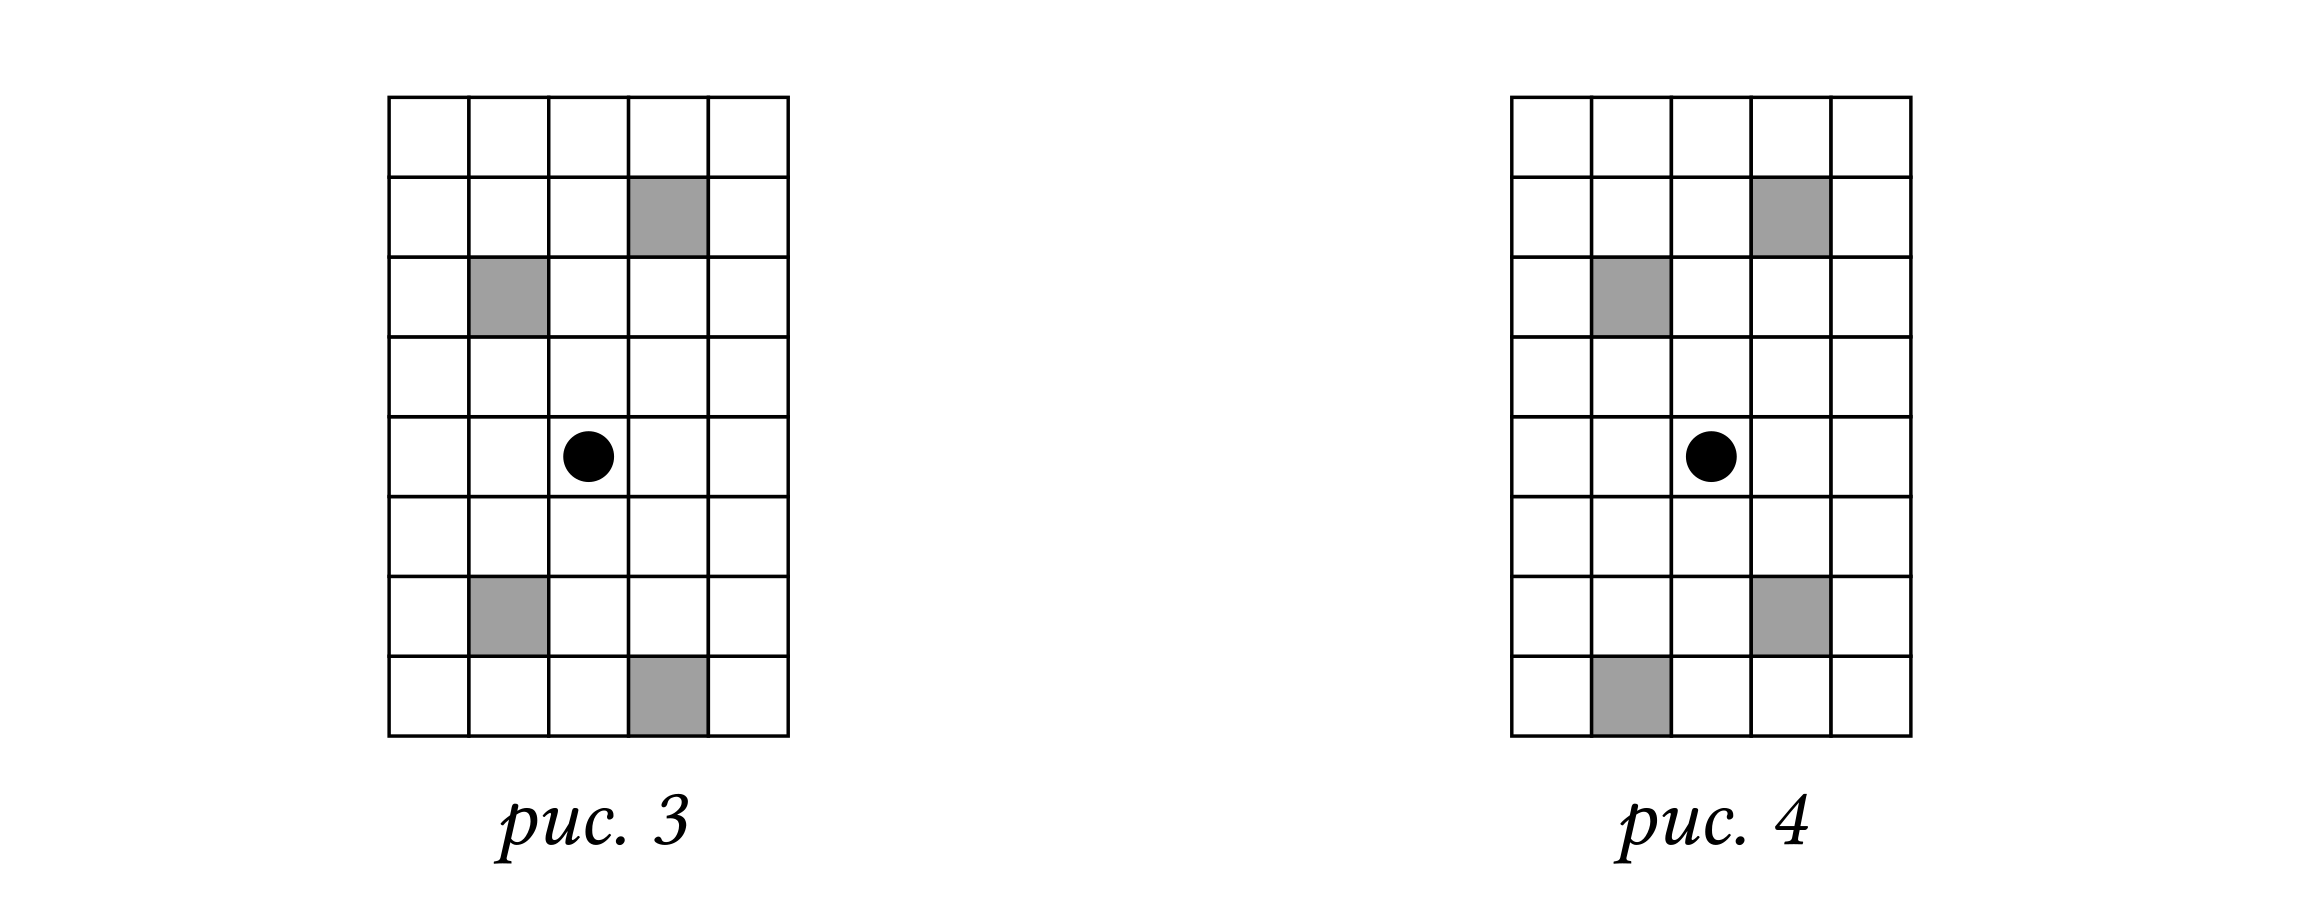
\includegraphics[width=8.5cm]{Figures/Corbleud.png}
\end{center}
